\documentclass[oneside,dutch]{tudelft-report}
\DeclareGraphicsExtensions{.pdf,.png,.jpg,.jpeg}
%\usepackage[numbered, framed]{mcode}
\usepackage{subcaption}
\usepackage{float}
\usepackage[dutch]{babel}
\usepackage{calc}  
\usepackage{enumitem}  
\usepackage{tabto}
\usepackage{adjustbox}
\usepackage{blindtext}
\usepackage{listings}
\usepackage{caption}

\begin{document}

\frontmatter

\title{Mid-term report}
\author{Projectgroep A5}
\affiliation{TU Delft}
\maketitle
\chapter{Samenvatting}


\chapter{Inleiding}
\newpage

\chapter{Probleemstelling}
\newpage

\chapter{Systeem overzicht}
\newpage

\chapter{Besturing}
Ons systeem wordt gespeeld doormiddel van 2 soorten besturing. De Ultrasone en de Button. De speler kan de modus selecteren doormiddel van een switch. Deze data van de buttons en de ultrasone worden verwerkt door een Arduino. Er is gekozen voor deze optie omdat de Arduino via SPI werkt. Hierdoor kan de SPI code getest worden en kunnen we het aantal pinnen dat gebruikt wordt laag houden. 

\subsection{Ultrasone}
Een unieke uitdaging van ons project is de Ultrasone besturing, de besturing werkt door middel van een (ultrasone)sensor aan de rechterzijde van de speler. Deze sensor meet met een speel ruimte van 75cm elke 11 milliseconde. Het aansturen van de ultrasone sensoren gaat doormiddel van een 2ms lange pulse op de IN-pin. Dit is de trigger van de SRF-04(de door ons gekozen ultrasone sensor). Hierna verzend de sensor zijn pulse, op dat moment wordt de OUT-pin ook hoog. Deze blijft hoog tot de gereflecteerde pulse weer binnen komt. Deze tijd wordt gedeeld door 2 omdat het geluid zowel de afstand heen als terug moet afleggen. Deze tijd wordt vervolgens geschaald naar afstand door hem door 29m/s(de snelheid van geluid in lucht) te delen. Hierna wordt de tijd teruggemapt(alles tussen de 0 en de 75 wordt terug geschaald naar 0 en 12). Deze waarde wordt voor player 2 4 bits geschoven naar links. En vervolgens wordt het signaal via de hierbovengenoemende SPI verstuurd naar de chip.

\subsection{Buttons}
Bij de buttons wordt een andere manier van werken gehanteerd, hier wordt de waarde van de plaatsvector onthouden(als integer). En naar gelang welke button geactiveerd wordt, wordt het signaal 1 verhoogd/verlaagd. Dit getal kan maximaal 12 bereiken en minimaal 0. Vervolgens wordt dit signaal voor player 2 ook verschoven, en daarna verzonden via SPI.

De getallen 0->12 voor player 1/2 zijn in gebruik, dit geeft ruimte om 13,14,15 te gebruiken voor andere doeleinde. 13 dient als getal om de Start van systeem aan te geven. 15 is de Reset van het systeem.
\newpage

\chapter{Blackbox}
\newpage

\chapter{ALU/PC}
\newpage

\chapter{VGA}
\newpage

\chapter{SPI}
Serial Peripheral Interface in het kort ook SPI genoemd is een de facto-standaard die ooit door Motorola bedacht is voor het communiceren met randapparatuur, zoals embedded systems, sensors en memory cards. Bij SPI heb je de master en de slave deze communiceren met elkaar via twee seriële datalijnen daarnaast is er nog een kloklijn die aangeeft wanneer er data overgedragen wordt. De kloklijn wordt aangestuurd door de master, dit houdt in dat de slave niet kan pauzeren en altijd data aan de master aan moet bieden. De standaard definieert enkel hoe de data van de master naar de slave en vice versa over wordt gedragen, niet hoe de data verwerkt wordt, dit heeft als gevolgd dat randapparatuur zelf nog moet definiëren hoe de communicatie verloopt.

\section{Functionele beschrijving}
De SPI module begint met zenden/ontvangen zodra het send signaal hoog is en stopt zodra er acht bits zijn verzonden/ontvangen, daarna kunnen de ontvangen bits uitgelezen worden en nieuwe bits in worden geladen om te verzenden. Het overbrengen van het shift register dat in de master zit naar de slave en vice versa deze shift registers zijn in een kring op elkaar aangesloten, waarbij altijd de meest significante bit wordt verzonden. Voor de communicatie met de slave wordt een slave klok signaal gegenereerd, de data overdracht is gesynchroniseerd ten opzicht van dit signaal. Data wordt gesampled op de opgaande klokflank en de data wordt geshift op de neergaande klokflank.

\section{Inputs en outputs}

\begin{figure}[H]
\center
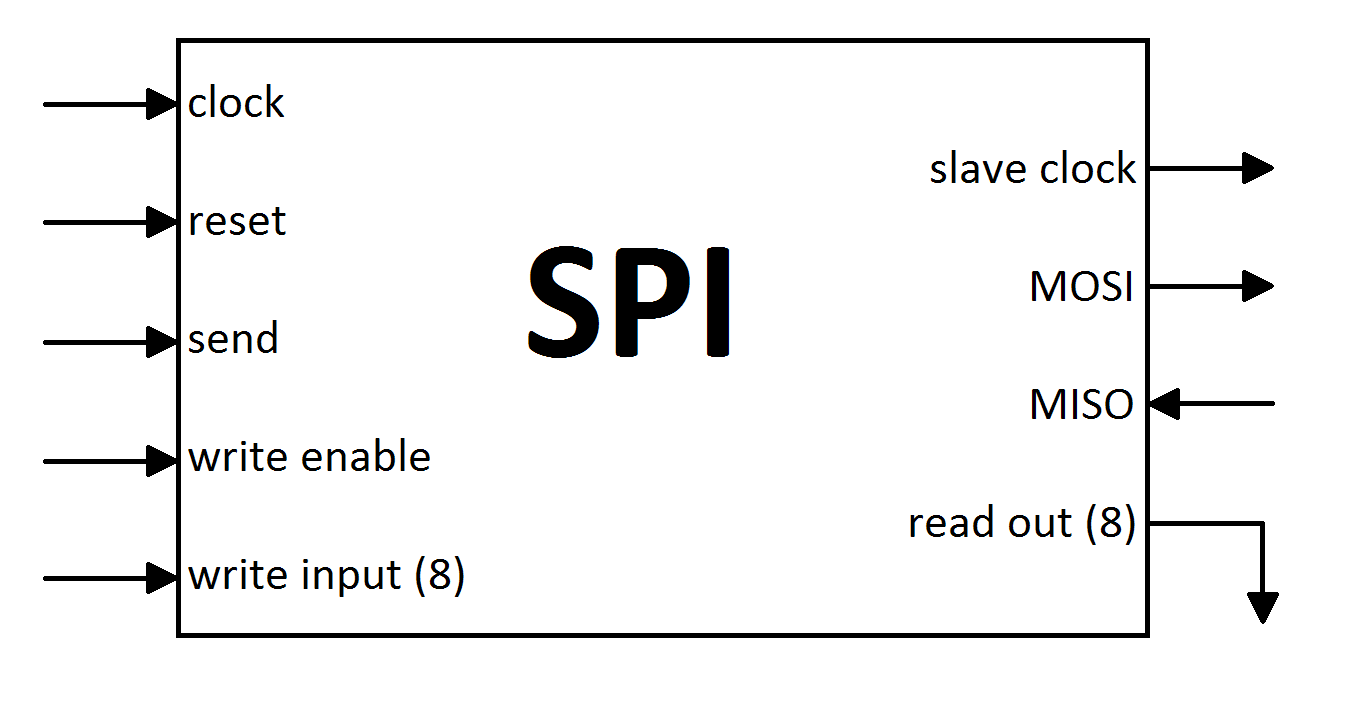
\includegraphics[width=9cm]{./spi_diagram}
\caption{Diagram of SPI circuit}
\label{spi-diagram}
\end{figure}

\begin{itemize}
\item Clock: het kloksignaal waarop de SPI draait, het slave clock signaal zal dezelfde frequency hebben als dit kloksignaal
\item Reset: de hoofd reset van de SPI
\item Send: de input die aangeeft wanneer er begonnen moet worden met zenden/ontvangen
\item Write\_enable: als deze hoog is zal write\_in(8) in het shift register geladen worden
\item Write\_in(8): de bits die naar het shift register worden geschreven als write\_enable hoog is
\item Read\_out(8): de waarde die in het shift register staat
\item Slave clock: het slave kloksignaal die de communicatie met de slave aanstuurt
\item MOSI: de datalijn van de master naar de slave
\item MISO: de datalijn van de slave naar de master
\end{itemize}

\section{Implementatie}
Voor de implementatie van de SPI is er voor gekozen om het in drie subsystemen op te delen:
\begin{itemize}
\item Counter: een simpele teller die de opgaande klokslagen van het slave clock signaal telt. 
\item Shift register: een shift register van acht bits die shift op de neergaande klokflank als het enable signaal hoog is en nieuwe waardes inlaad als de write enable hoog is. Het blokschema van het shift register is te zien in figuur \ref{shift-register-diagram}.
\item Control: een statemachine die er voor zorgt dat de SPI stopt met shiften na 8 klokslagen van de slave klok, zodat er tijd is om het register uit te lezen of nieuwe waarden in te laden. Het blokschema van Control is te zien in figuur \ref{control-diagram}.
\end{itemize}

Deze drie subsystemen zijn aan elkaar verbonden volgens het schema in figuur \ref{spi-system-diagram}.

\begin{figure}[H]
\centering
\begin{minipage}{.5\textwidth}
  \centering
  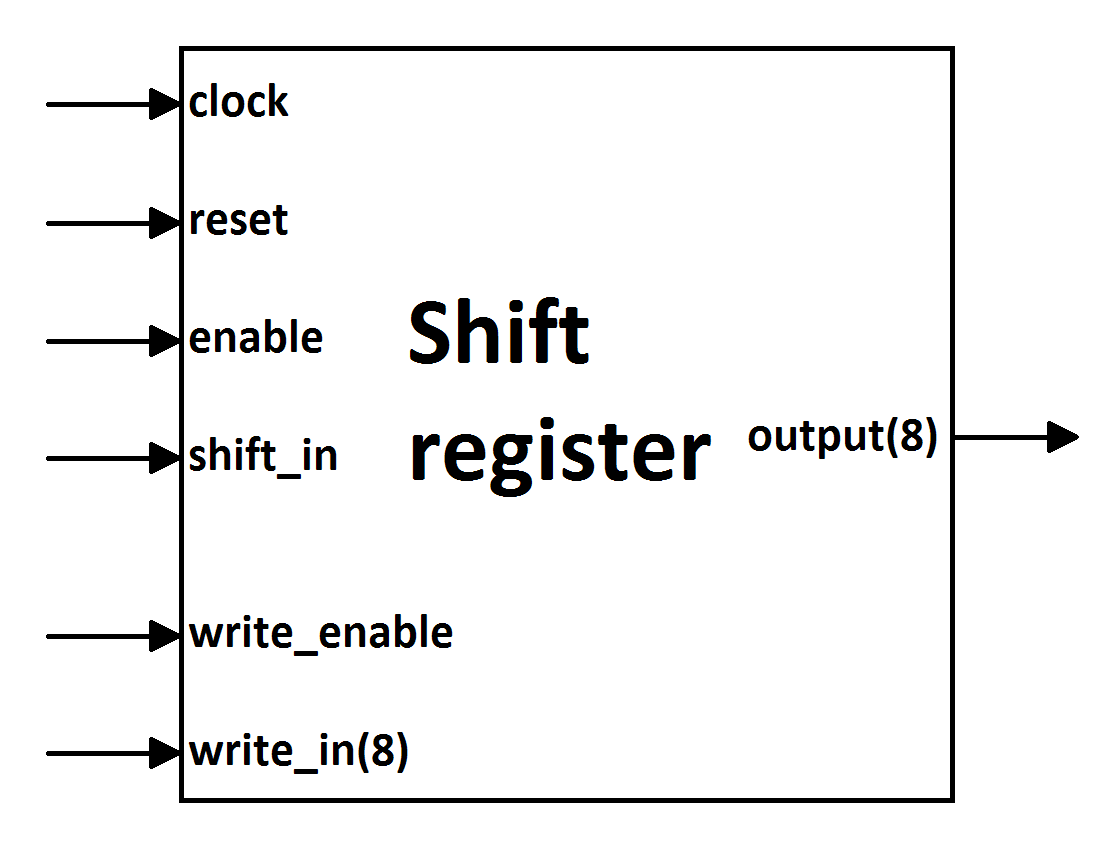
\includegraphics[width=7cm]{./shift_register_diagram}
  \captionof{figure}{Diagram van Shift regiser}
  \label{shift-register-diagram}
\end{minipage}%
\begin{minipage}{.5\textwidth}
  \centering
  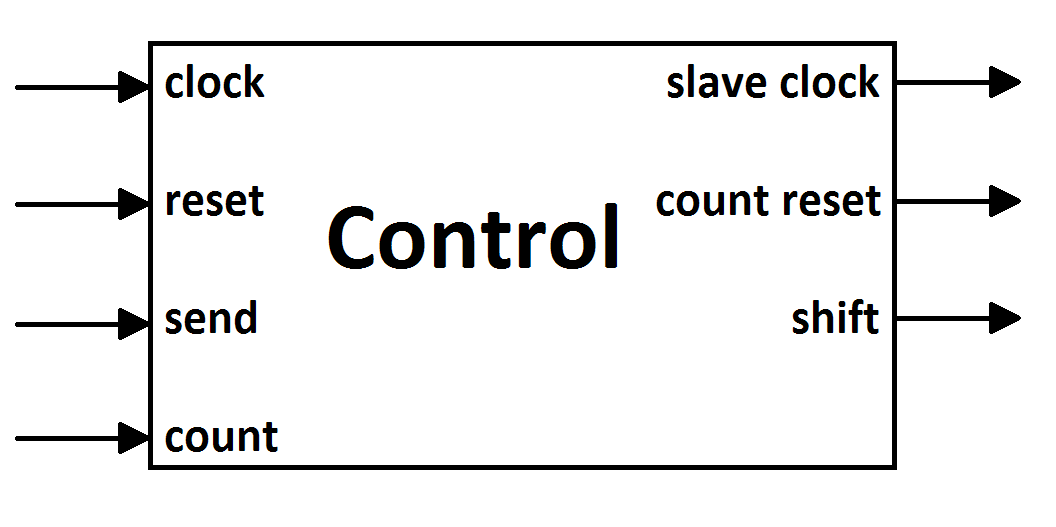
\includegraphics[width=9cm]{./control_diagram}
  \captionof{figure}{Diagram van Control} 
  \label{control-diagram}
\end{minipage}
\end{figure}

\begin{figure}[H]
\center
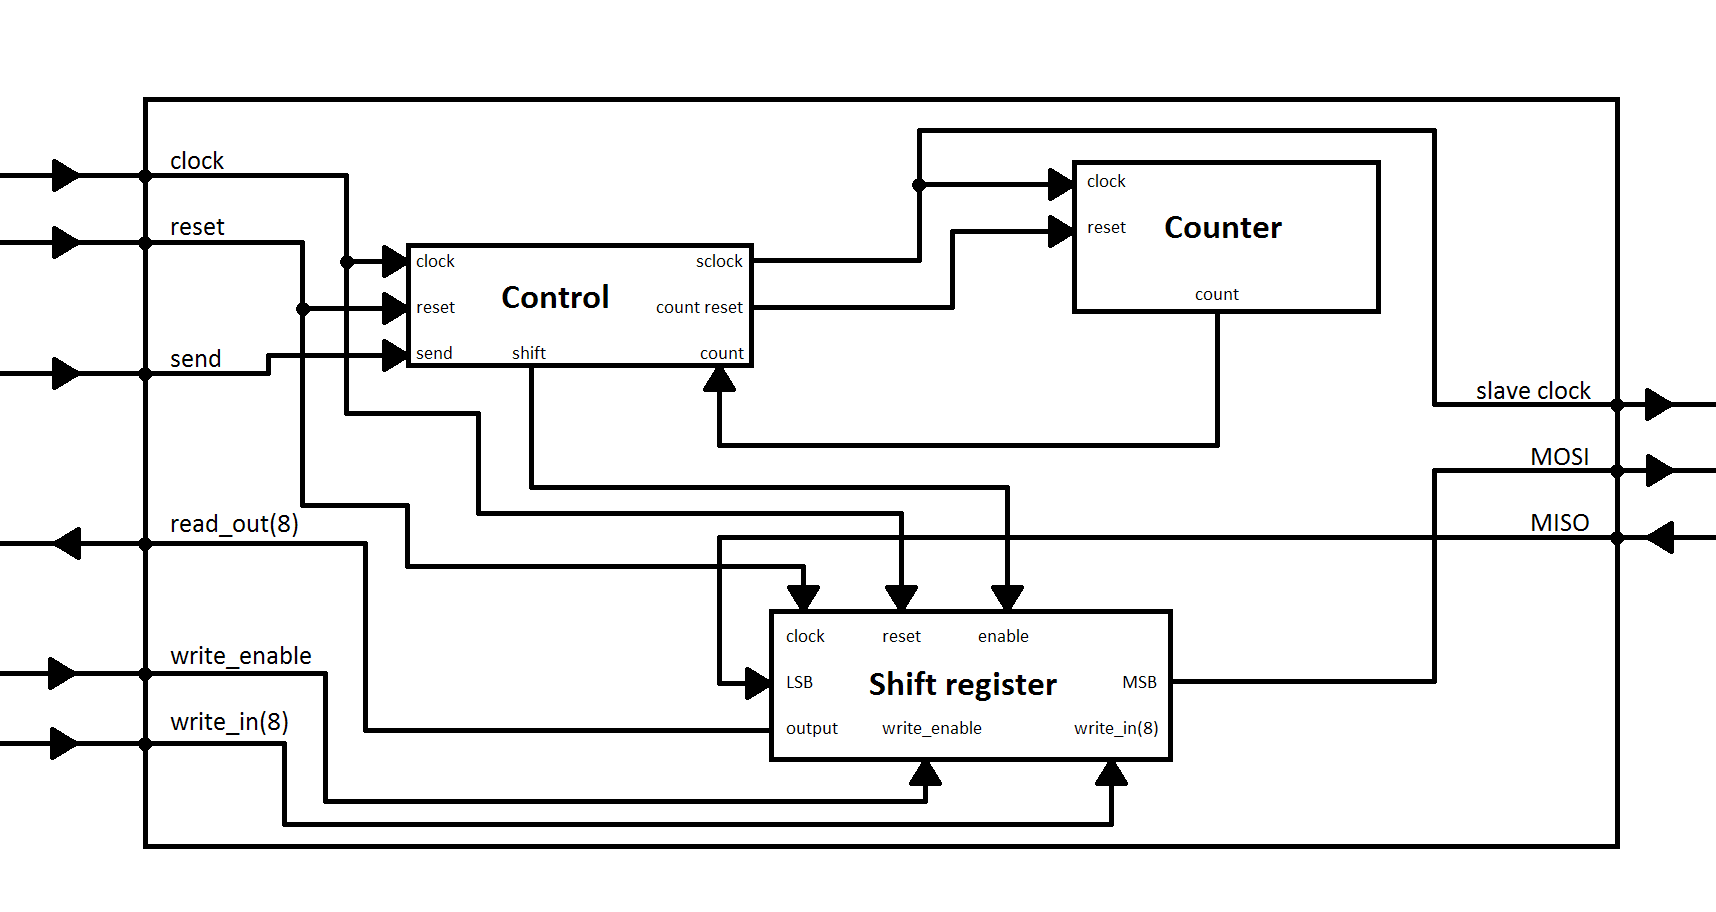
\includegraphics[width=14cm]{./spi_system_diagram}
\caption{Diagram van de verbinding van de componenten}
\label{spi-system-diagram}
\end{figure}

\newpage

\chapter{SD-kaart}
\newpage

\chapter{Game: Pong}

\end{document}